\documentclass{article}

\usepackage{fancyhdr}
\usepackage{extramarks}
\usepackage{amsmath}
\usepackage{amsthm}
\usepackage{amsfonts}
\usepackage{tikz}
\usepackage[plain]{algorithm}
\usepackage{algpseudocode}

\usetikzlibrary{automata,positioning}

%
% Basic Document Settings
%

\topmargin=-0.45in
\evensidemargin=0in
\oddsidemargin=0in
\textwidth=6.5in
\textheight=9.0in
\headsep=0.25in

\linespread{2.0}

\pagestyle{fancy}
\lhead{\hmwkAuthorName}
\chead{\hmwkClass\ (\hmwkClassInstructor\ \hmwkClassTime)}
\rhead{\firstxmark}
\lfoot{\lastxmark}
\cfoot{\thepage}

\renewcommand\headrulewidth{0.4pt}
\renewcommand\footrulewidth{0.4pt}

\setlength\parindent{0pt}

%
% Create Problem Sections
%

\newcommand{\enterProblemHeader}[1]{
    \nobreak\extramarks{}{Problem \arabic{#1} continued on next page\ldots}\nobreak{}
    \nobreak\extramarks{Problem \arabic{#1} (continued)}{Problem \arabic{#1} continued on next page\ldots}\nobreak{}
}

\newcommand{\exitProblemHeader}[1]{
    \nobreak\extramarks{Problem \arabic{#1} (continued)}{Problem \arabic{#1} continued on next page\ldots}\nobreak{}
    \stepcounter{#1}
    \nobreak\extramarks{Problem \arabic{#1}}{}\nobreak{}
}

\setcounter{secnumdepth}{0}
\newcounter{partCounter}
\newcounter{homeworkProblemCounter}
\setcounter{homeworkProblemCounter}{1}
\nobreak\extramarks{Problem \arabic{homeworkProblemCounter}}{}\nobreak{}

%
% Homework Problem Environment
%
% This environment takes an optional argument. When given, it will adjust the
% problem counter. This is useful for when the problems given for your
% assignment aren't sequential. See the last 3 problems of this template for an
% example.
%
\newenvironment{homeworkProblem}[1][-1]{
    \ifnum#1>0
        \setcounter{homeworkProblemCounter}{#1}
    \fi
    \section{Problem \arabic{homeworkProblemCounter}}
    \setcounter{partCounter}{1}
    \enterProblemHeader{homeworkProblemCounter}
}{
    \exitProblemHeader{homeworkProblemCounter}
}

%
% Homework Details
%   - Title
%   - Due date
%   - Class
%   - Section/Time
%   - Instructor
%   - Author
%

\newcommand{\hmwkTitle}{Homework\ \#5}
\newcommand{\hmwkDueDate}{September 25th, 2015}
\newcommand{\hmwkClass}{Differential Equation}
\newcommand{\hmwkClassTime}{Section 061}
\newcommand{\hmwkClassInstructor}{Professor Heather Lee}
\newcommand{\hmwkAuthorName}{Yao Xiao}

%
% Title Page
%

\title{
    \vspace{2in}
    \textmd{\textbf{\hmwkClass:\ \hmwkTitle}}\\
    \normalsize\vspace{0.1in}\small{Due\ on\ \hmwkDueDate\ at 3:10pm}\\
    \vspace{0.1in}\large{\textit{\hmwkClassInstructor\ \hmwkClassTime}}
    \vspace{3in}
}

\author{\textbf{\hmwkAuthorName}}
\date{}

\renewcommand{\part}[1]{\textbf{\large Part \Alph{partCounter}}\stepcounter{partCounter}\\}

%
% Various Helper Commands
%

% Useful for algorithms
\newcommand{\alg}[1]{\textsc{\bfseries \footnotesize #1}}

% For derivatives
\newcommand{\deriv}[1]{\frac{\mathrm{d}}{\mathrm{d}x} (#1)}

% For partial derivatives
\newcommand{\pderiv}[2]{\frac{\partial}{\partial #1} (#2)}

% Integral dx
\newcommand{\dx}{\mathrm{d}x}

% Alias for the Solution section header
\newcommand{\solution}{\textbf{\large Solution}}

% Probability commands: Expectation, Variance, Covariance, Bias
\newcommand{\E}{\mathrm{E}}
\newcommand{\Var}{\mathrm{Var}}
\newcommand{\Cov}{\mathrm{Cov}}
\newcommand{\Bias}{\mathrm{Bias}}

\begin{document}

\maketitle

\pagebreak

\begin{homeworkProblem}
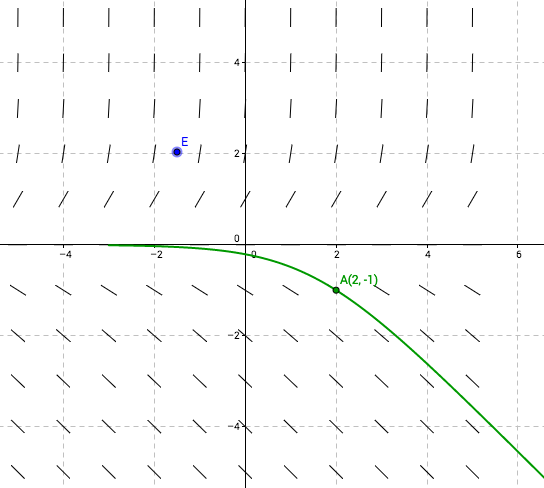
\includegraphics[scale=0.7]{image1.png} \\
From this sketch it appears that solutions that start “near” y = 0 all move away from it as t increases, so it's unstable.
\end{homeworkProblem}

\begin{homeworkProblem}
\( dy/dx=\alpha y(1-y) \) \\
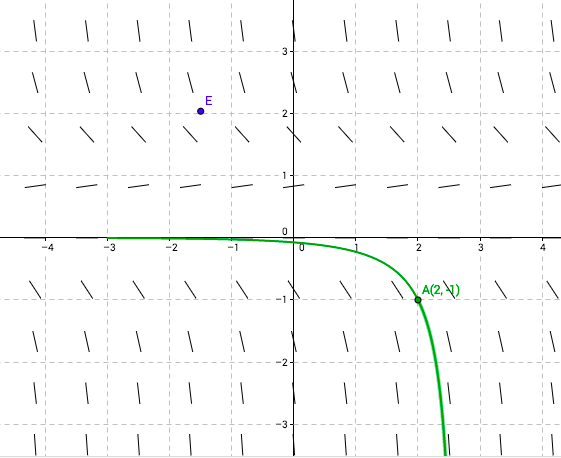
\includegraphics[scale=0.7]{image2.png} \\
From this sketch it appears that solutions that start “near” y = 0 all move away from it as t increases, so it's unstable.  solutions that start “near” y = 0 all move towards it as t increases, so it's asymptotically stable

2. \\
\[
	\begin{split}
		\int \frac{1}{y(1-y)}dy &= \int \alpha  dt \\
		 ln(y) - ln(1-y) &=\alpha t+C \\
		 \frac{y}{1-y} &=Ae^{\alpha t} \\
		 A &=\frac{y_0}{1-y_0} \\		
		 \frac{y}{1-y} &= \frac{y_0}{1-y_0}e^{\alpha t} \\
		 y &= \frac{ y_0 e^{\alpha t}}{y_0 e^{\alpha t}+1-y_0} \\
	\end{split}
\]

When \( t \to \infty, y \to 1 \) 

\end{homeworkProblem}

\begin{homeworkProblem}
1.The equilibrium solutions should be -2,4,8

2. When y=-2, it's asymptotic stable
When y=4, it's semi-stable
When y=8, it's not stable
\end{homeworkProblem}
\begin{homeworkProblem}
Since \[ \frac{\partial M(x)}{\partial y}=\frac{\partial N(y)}{\partial x}=0 \]

So it's exact equation
\end{homeworkProblem}
\begin{homeworkProblem}
\[ \frac{dw}{dt}=\frac{2tw}{w^2-t^2}\]
Let w=at, 
dw/dt=a+t(da/dt) \\
\((2tw) / (w^2 - t^2)=(2at^2)/((at)^2-t^2) 
=2a/(a^2-1) \)

\[
\begin{split}
a+t\frac{da}{dt} &=\frac{2a}{a^2-1} \\
t\frac{da}{dt} &=\frac{2a-a(a^2-1)}{a^2-1}\\
t\frac{da}{dt} &=\frac{2a-a(a^2-1)}{a^2-1}\\
\frac{3a-a^3}{a^2-1} &= t\frac{da}{dt} \\
\frac{a^2-1}{3a-a^3}da &= \frac{1}{tdt} \\
t(a) &=\frac{C}{\sqrt[3]{a(3-a^2)}} \\
t^3a(3-a^2) &= C\\
 a &= w/t \\
 wt^2(3-w^2/t^2)&=C  \\
 w&=\frac{C}{3t^2-w^2}
\end{split}
\]
\end{homeworkProblem}

\begin{homeworkProblem}
a)
\[
\begin{split}
y'&=1-t+y  \\
y(t_0)&=y_0 \\
(e^{-t}y)'&=(1-t)e^{-t}
\end{split}
\]
Integrate both side, we get \(e^{-t}y=te^{-t}+C \)
So \[
y(t)=t+(y_0-t_0)e^{t-t_0}
\]

b)
\[ 
\begin{split}
y_k=y_{k-1}+hf(k-1) \\
f(k-1) = 1-t+y \\
y_k=(1+h)y_{k-1}+h-ht_{k-1} \\
\end{split}
\]
\[y_k = y_{k−1} + h(1 − t_{k−1} + y_{k−1}) = (1 + h)y_{k−1} + h − ht_{k−1} \]

d) when \(  h=\frac{t-t_0}{n}\) \\
\[ y_n=(1+h)^n(y_0-t_0)+t=(1+\frac{t-t_0}{n})^n(y_0-t_0)+t \]

since \(	n \to \infty  \), the upper formula becomes \(y_n=(1+\frac{t-t_0}{n})^n(y_0-t_0)+t \)
\[
= e^{t-t_0}(y_0-t_0)+t
\]
\end{homeworkProblem}

\begin{homeworkProblem}
\[
\begin{split}
	y'&=-2y+e^{-t}\\
	y=e^-{t}+c
 	C &= 0 \\
	y(t)=e^{-t}	\\
\end{split}
\]
So \( y(1)=\frac{1}{e} \)

2. Using the following code:
\begin{verbatim}
n=1;
while (1)
[x,y]=eul('fcn1',[0,1],1,1/n);
if abs(y(end)-1/exp(1))<0.05
     disp(n);
     break;
end
n=n+1;
end

\end{verbatim}

We get the result:
\begin{verbatim}
x =

     0
     1


y =

     1
     0


x =

         0
    0.5000
    1.0000


y =

    1.0000
    0.5000
    0.3033


x =

         0
    0.3333
    0.6667
    1.0000


y =

    1.0000
    0.6667
    0.4611
    0.3248
\end{verbatim}

so n=3
\end{homeworkProblem}

\begin{homeworkProblem}
\[
\begin{split}
	y'&=2y-3e^{-t}\\
	y'-2y&=-3e^{-t} \\
	(e^{-2t}y)'&=-3e^{-3t} \\
	e^{-2t}y=e^{-3t}+C \\
 	C &= 0 \\
	y(t)=e^{-t}	\\
\end{split}
\]
So \( y(1)=\frac{1}{e} \)

2. Using the same code as above, we get \(n=22\)

\end{homeworkProblem}

\begin{homeworkProblem}
1. Since 
\[
\frac{dy}{dt}=\frac{d\int _{a}^{t} e^{-u^2}}{dt}
\]
Using fundamental theory of calculus.
We get
\[
\frac{dy}{dt}=f(t)=e^{-t^2}
\]

2. plug in using the same code for problem 7
\begin{verbatim}
ans =

         0         0
    0.5000    0.5000
    1.0000    0.8894
    1.5000    1.0733
    2.0000    1.1260
\end{verbatim}

So f(2)=1.1260
\end{homeworkProblem}



\end{document}
